
\documentclass[main.tex]{subfiles}
\begin{document}

\section{CSS}
CSS (zkratka z anglického Cascading Style Sheet, v češtině kaskádové styly) je jazyk, definující způsob zobrazení elementů na HTML, XHTML nebo XML stránce. Hlavní myšlenkou je oddělit obsah a strukturu dokumentu od jeho vizuální podoby, jako barvy, rozložení a fontů. Toto oddělení také umožňuje použít stejný vizuální vzhled pro více HTML stránek. Autorem myšlenky oddělit obsah od vzhledu je norský programátor Håkon Wium Lie. Nyní je publikovaný pod organizací W3C.  

\subsection{Specifikace}
\begin{quote} \textit{"Definice kaskádových stylů sestává z několika pravidel. Každé pravidlo obsahuje selektor a blok deklarací. Každý blok deklarací pak obsahuje deklarace oddělené středníky ; a každá deklarace sestává z identifikátoru vlastnosti, následuje dvojtečka : a hodnota vlastnosti. Nepovinně ještě může následovat označení !important, které zvýší sílu deklarace."} \cite{web:wik:cz:css} \end{quote} 

	\subsubsection{Selektory}
Pravidla jsou na HTML elementy uplatňována podle selektorů, a základní můžeme rozdělit následujícím způsobem.
\begin{itemize}
	\item Selektor pro elementy jednoho typu. Například pro nadpis třetí úrovně  $<h3>$.
		\begin{figure}[h]
			\centering
			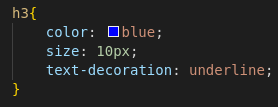
\includegraphics[width=.3\textwidth]{./css/h3.png}
			\caption{Znazornění třídy}
		\end{figure}
		Zahrneme-li toto pravidlo do HTML, všechny nadpisy 3. úrovně budou modrou barvou, velikosti 10 pixelů a podtržené.
	\item Elementy s konkrétním atributem - názvem třídy nebo id.
		\begin{itemize}
			\item Podle atributu id, jež musí být unikátní v celém dokumentu. Pravidla s tímto selektorem se použijí pro nejvýše jeden element a zapisují se \textit{idname}. %dat pred id_name #
			\item Podle atributu class. Ten nemusí být unikátní. Zapisují se \textit{.classname}.
		\end{itemize}


		\begin{figure}[h]
			\centering
			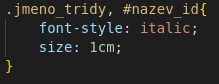
\includegraphics[width=.3\textwidth]{./css/classid.png}
			\caption{Znazornění třídy}
		\end{figure}
		Pravidla mohou mít více selektorů oddělených čárkou. Pro všechny elementy s atributem \textit{class = "jmenotridy"} a unikátní element s atributem \textit{id ="nazevid"}, bude text psán kurzivou o velikost 1 cm.
	\item Elementy v závislosti na jejich umístění v hierarchii dokumentu. Například pravidla se selektorem \textit{body>div} budou aplikována pouze na elementy \textit{div}, které jsou přímým potomkem elementu \textit{body}. Neplatil by tedy pro \textit{div} uzavřený v elementu \textit{p}, uzavřeném v elementu \textit{body}.
\end{itemize}
Výše vyjmenované sektory však nejsou kompletní. Existuje množství dalších selektorů. \cite{web:cz:selektory}

\subsection{Zahrnutí do HTML}
Existují tři možnosti, kde zapisovat CSS pravidla, aby byla zahrnuta do HTML.
\subsubsection{inline zápis}
Tento zápis je připsán ke konkrétnímu elementu vedle zápisu jeho atributů.
		\begin{figure}[h]
			\centering
			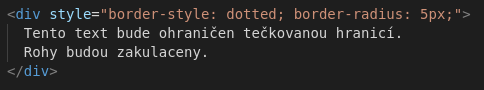
\includegraphics[width=.6\textwidth]{./css/inline.png}
			\caption{popisek}
		\end{figure}
Tento zápis se nedoporučuje používat, jelikož potlačuje výhody CSS - oddělení obsahu a vizuální podoby.

\subsubsection{Zápis v hlavičce}
CSS pravidla jsou zapsána v hlavičce HTML dokumentu do tagu $<head>$. Nevýhodou je aplikace pravidel pouze na jeden konkrétní dokument.
		\begin{figure}[h]
			\centering
			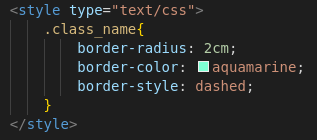
\includegraphics[width=.3\textwidth]{./css/header.png}
			\caption{Znazornění třídy}
		\end{figure}
\subsubsection{Externí CSS soubor}
Nečastěji používaným způsobem je deklarace pravidel v externím souboru. Ten může být s HTML dokumentem provázán tagem \textit{$<link>$}.
		\begin{figure}[h]
			\centering
			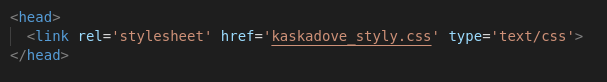
\includegraphics[width=.6\textwidth]{./css/extern.png}
			\caption{Znazornění třídy}
		\end{figure}
Atribut \textit{href} udává relativní cestu k souboru, atribut \textit{type} říká prohlížeči, aby daný soubor interpretoval jako CSS. 
Další možností je připojení externího souboru pomocí http hlavičky.
Poslední možností, jak připojit externí soubor je tagem \textit{$<style>$} s pravidlem \textit{@important}.



%\subsection{Blok deklarací}
%Blok deklarací uvedený selektorem obsahuje několik uspořádaných dvojic - \textit{identifikátor vlastnosti : hodnota vlastnosti}. Identifikátory vlastností jsou typicky anglické názvy vlastností, jako color, border, font-family.

%Tento blok deklarací nastavuje barvu písma na modrou identifikátorem color, atd.. dopsat. 


\end{document}
